\documentclass{article}

\usepackage[final]{neurips_2019}

\usepackage[utf8]{inputenc}
\usepackage[T1]{fontenc}
\usepackage{hyperref}
\usepackage{url}
\usepackage{booktabs}
\usepackage{amsfonts}
\usepackage{nicefrac}
\usepackage{microtype}
\usepackage{graphicx}
\usepackage{xcolor}
\usepackage{lipsum}

\newcommand{\note}[1]{\textcolor{blue}{{#1}}}

\title{
  Predicting Block Copolymer Properties Using Graph Neural Networks \\
  %\vspace{1em}
  %\small{Project Category:} \\
}

\author{
  Name: Thomas Little\\
  SUNet ID: 06510735\\
  Department of Civil and Environmental Engineering \\
  Stanford University \\
  \texttt{tjlittle@stanford.edu} \\
  % Examples of more authors
  %\And
  %Name: \\
  %SUNet ID: \\
  %Department of Computer Science \\
  %Stanford University \\
  %\texttt{name@stanford.edu} \\
}

\begin{document}

\maketitle

% \begin{abstract}
%   Required for final report
% \end{abstract}


\section{Application Domain}
Block copolymers are a class of polymer that are composed of two or more distinct monomers chemically joined to create a single molecule. The materials block copolymers form exhibit a wide range of microstructures and properties that make them useful for a variety of applications including materials science, nanotechnology, and biomedical engineering. The study of block copolymers, however, is often limited by the high computational cost of traditional self-consistent field theory simulations. These simulations are valuable tools for the characterization of block copolymers, however, due to their iterative nature it becomes difficult to perform large-scale simulations in a reasonable amount of time.

The goal of this study is to predict the phase behavior of block copolymers using a graph neural network architecture. Recent work has shown the ability of random forest models to closely approximate block copolymer phase behavior with greatly reduced computation time\cite{RandForest}. This approach, however, is not adequately able to capture more geometrically complex copolymer structures, therefore the use of a graph neural network aims to remedy this.

There is an open source database of block copolymer phase behavior that was published in 2021 by a research group at MiT\cite{BCDB}. This database has over 5,300 block copolymer melt phase measurements that have been mined from literature and manually curated. This dataset was chosen due to its availability and size. There are few databases that contain such an exhaustive list of block copolymers and their respective properties, especially those that contain the properties needed to calculate phase behavior.

The input variables considered in this study will be the block copolymers geometries, which will be represented as a graph, where the nodes are monomers and their respective properties and the connections denote the bonds between these blocks. The previously mentioned database contains these monomers and their properties, along with known copolymer geometries. This information will be used to calculate miscibility using existing methods, specifically, for each copolymer in the dataset the Flory-Huggins parameter and volume fraction will be calculated. These parameters will be used to identify where each copolymer falls on the diblock copolymer phase diagram. These calculations will be considered ground-truth values and the accuracy of the model will be determined by how closely a GNN can replicate these properties. If the model is unable to accurately predict the Flory-Huggins or volume fraction parameters using a regression output, a classification approach can be explored, by changing the output to a multi-class classification and instead identifying which domain of the phase diagram each copolymer exists in.

\section{Graph ML Techniques}

Similar work has been conducted by the Olsen group at MiT\cite{RandForest} using random forest architectures to predict diblock copolymer phase behavior. The key difference in this approach is the machine learning framework used for prediction. Due to the constraints of input features in forest based approaches, the diblock copolymers were represented using a one-dimensional BigSMILES\cite{BigSMILES} framework of copolymer representation. While this framework is able to abstract block copolymers into an input string suitable for random forest architectures, some of the structure of the block copolymers is lost in this approach. A graph-based model will obviate these abstractions, leading to more accurate representations.

This study will use inductive modeling methods to ensure that the model can generalize to unseen copolymer structures. Initial models that will be considered are graph convolutional networks (GCNs) and graph attention networks (GATs) as both of these frameworks are well-suited for capturing relationships between nodes in asymmetric graph structures. A GCN will likely by used as a baseline model to get initial results while the GAT will be implemented for further model refinement if the GCN does not perform well. The GAT will likely have increased performance due to its ability to focus attention on characteristics of the copolymers that may have significant impact on phase behavior. These two specific network frameworks were chosen because they are capable of handling very asymmetric graphs, which is fitting for copolymers as their chain structures can become very long with minimal branching.

 \section{Conclusion}
The current proposal is to characterize diblock copolymer phase behavior, with the end goal being to correctly predict and classify diblock copolymers phase behavior according to the currently accepted phase diagram, as seen below. If the task of mapping diblock copolymers according to their phase diagram is achievable, a further improvement will be to look into triblock and n-block copolymer phase prediction and classification.

\begin{figure}[h]
\caption{Example of Diblock Copolymer Phase Diagram\cite{RandForest}}
\centering
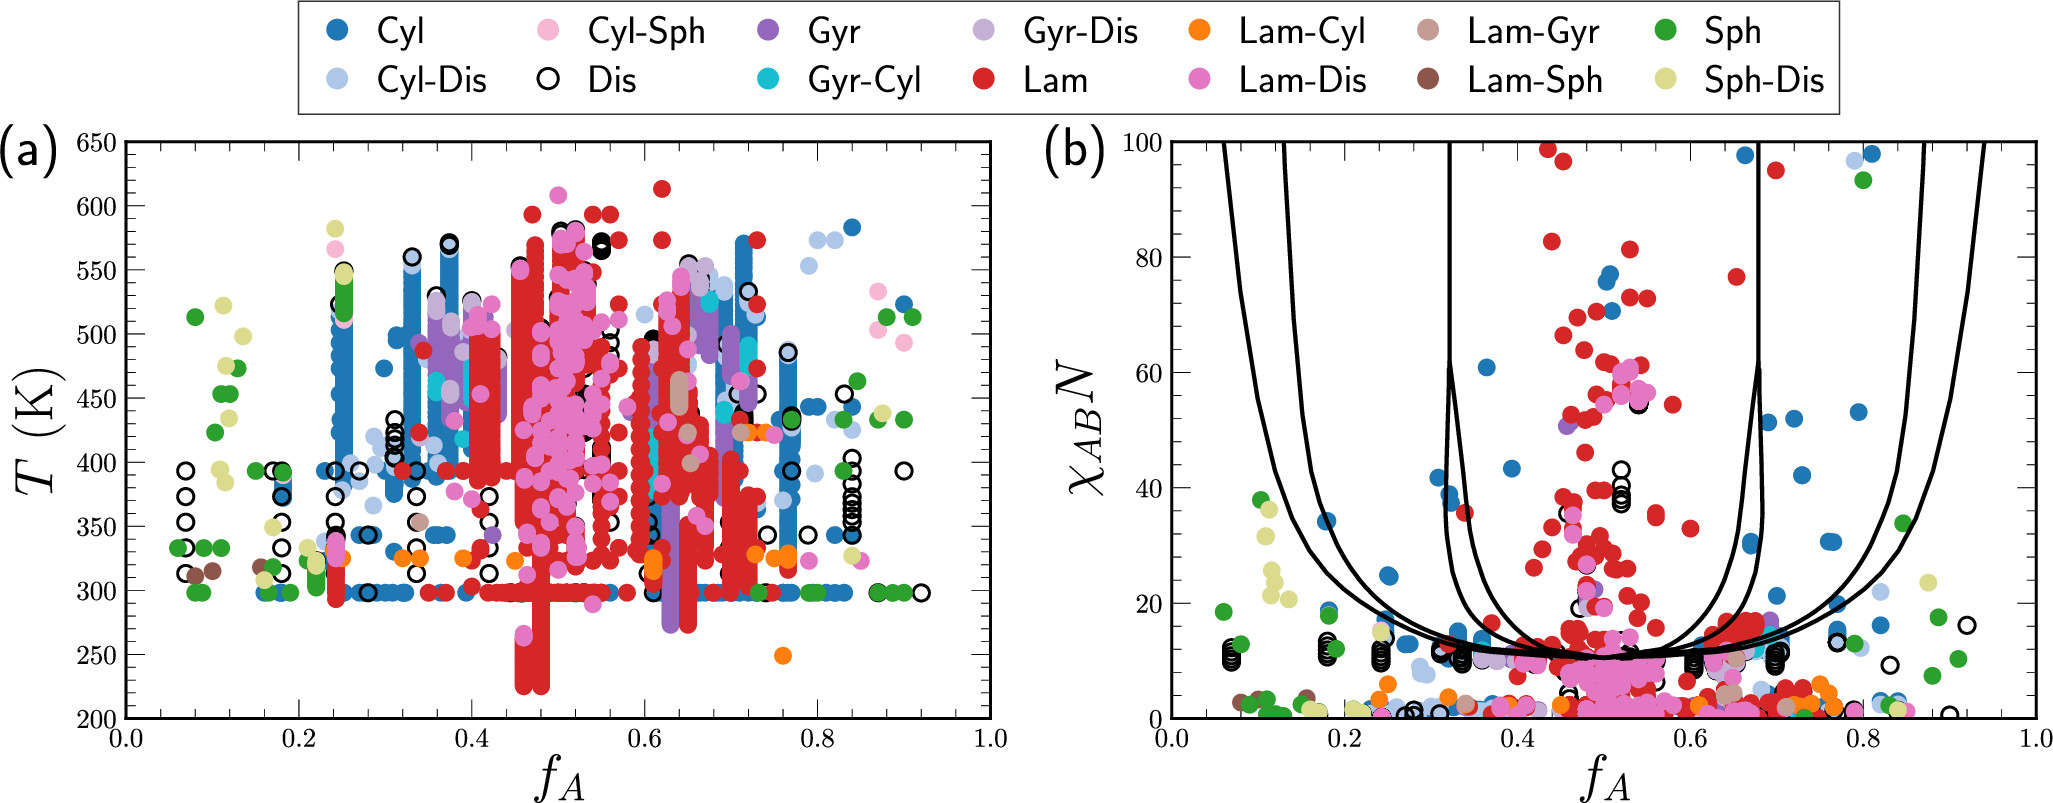
\includegraphics[width=\textwidth]{template/images_large_mz1c00521_0001.jpeg}
\end{figure}


\bibliographystyle{unsrt}
\bibliography{references}

\end{document}
